\chapter{Step}

%--------1---------2---------3---------4---------5---------6---------7---------8
In una elaborazione di uno step in generale abbiamo una (o più) origine dati
(tipicamente un file, ma non solo), una (o più) destinazione dati (tipicamente
un file, ma non solo) e un processo elaborativo che prende i dati dalla origine,
li trasforma in modo da poterli scrivere nella destinazione.

%--------1---------2---------3---------4---------5---------6---------7---------8
Nel caso che ci siano più origini dati, è il processo elaborativo che deve
decidere da quale origine leggere, e non è possibile parallelizzare il processo
elaborativo.

%--------1---------2---------3---------4---------5---------6---------7---------8
Nel caso di una singola origine dati il processo elaborativo non richiede una
logica di lettura; la lettura dalla origine dati può essere fatta dalla
infrastruttura, e il processo elaborativo può essere parallelizzato.
In questo caso, nelle destinazioni dati può essere mantenuta o meno la
sequenzialità della origine dati (dipende dalla implementazione della
parallelizzazione).

%--------1---------2---------3---------4---------5---------6---------7---------8
Per gestire in modo generico le sorgenti e destinazioni dati vengono usate le
classi
\begin{itemize}
    \item \hyperref[sec:srcRes]{\texttt{SourceResource}} sorgente dati
    \item \hyperref[sec:snkRes]{\texttt{SinkResource}} destinazione dati
\end{itemize}

%--------1---------2---------3---------4---------5---------6---------7---------8
Nel caso che sia presente una sola sorgente dati la parte elaborativa può
produrre una tupla e sarà la infrastruttura a inviare i dati alle destinazioni,
in questo caso il formato elaborativo è:
%--------1---------2---------3---------4---------5---------6---------7---------8
\begin{elisting}[!htb]
\begin{javacode}
    Pgm.from(src).into(snk1,snk2).forEach(it -> { ... });
\end{javacode}
\caption{elaborazione $1\mapsto N$}
\label{lst:processTuple}
\end{elisting}


%--------1---------2---------3---------4---------5---------6---------7---------8
in alternativa alla parte elaborativa oltre al valore di input vengono forniti i
\texttt{Consumer} per scrivere direttamente in dati sulle corrispondenti
destinazioni, il questo caso il formato elaborativo è:
%--------1---------2---------3---------4---------5---------6---------7---------8
\begin{elisting}[!htb]
\begin{javacode}
    Pgm.from(src).into(snk1,snk2).forEach((it,wr1,wr2) -> { ... });
\end{javacode}
\caption{elaborazione writer}
\label{lst:processWriter}
\end{elisting}
%--------1---------2---------3---------4---------5---------6---------7---------8
entrambi i formati possono essere parallelizzati, ma solo il primo permette una
implementazione che mantiene l'\,ordine dei dati originale.

%--------1---------2---------3---------4---------5---------6---------7---------8
Nel caso che siano presenti più di una sorgente dati, alla parte elaborativa
vengono forniti i \texttt{Supplier} per leggere i dati dalle origini, e i
\texttt{Consumer} per scrivere i dati, in questo caso il formato elaborativo è:
%--------1---------2---------3---------4---------5---------6---------7---------8
\begin{elisting}[!htb]
\begin{javacode}
    Pgm.from(src1, src2).into(snk1, snk2).proceed((rd1, rd2, wr1, wr2) -> { ... });
\end{javacode}
\caption{elaborazione reader-writer}
\label{lst:pullProcess}
\end{elisting}


%--------1---------2---------3---------4---------5---------6---------7---------8
Nel caso di una sorgente possono essere usate da 0 a 12 destinazioni,
nel caso di più sorgenti, da 2 a 3, si possono avere da 0 a 8 destinazioni.

%--------1---------2---------3---------4---------5---------6---------7---------8
Il codice di questa libreria è interamente generato dal plugin con le
configurazioni di default, lst.~\ref{lst:plugin-conf}.

\begin{elisting}[!htb]
\begin{xmlcode}
<plugin>
    <groupId>io.github.epi155</groupId>
    <artifactId>promethium-batch-pgm-maven-plugin</artifactId>
    <version>...</version>
    <executions>
        <execution>
            <goals>
                <goal>generate</goal>
            </goals>
        </execution>
    </executions>
    <configuration>
        <rangeOut>0..12</rangeOut>
        <muRangeInp>2,3</muRangeInp>
        <muRangeOut>0..8</muRangeOut>
    </configuration>
</plugin>
\end{xmlcode}
\caption{plugin per generare il codice della libreria}
\label{lst:plugin-conf}
\end{elisting}

%--------1---------2---------3---------4---------5---------6---------7---------8
Nel caso di elaborazione sequenziale la separazione della elaborazione in una
parte dedicata alla lettura dei dati, una dedicata alla scrittura dei dati e una
specifica per la elaborazione dei dati, non offre particolari vantaggi.

%--------1---------2---------3---------4---------5---------6---------7---------8
Questa separazione è propedeutica alla elaborazione parallela.
Una elaborazione sequenziale nella forma~\ref{lst:pushSeq}
%--------1---------2---------3---------4---------5---------6---------7---------8
\begin{elisting}[!htb]
\begin{javacode}
    Pgm.from(src).into(...).forEach(...);
\end{javacode}
\caption{elaborazione sequenziale}
\label{lst:pushSeq}
\end{elisting}
%--------1---------2---------3---------4---------5---------6---------7---------8
può essere trasformata nella forma parallela~\ref{lst:pushMt}, sostituendo il
\texttt{forEach} in \texttt{forEachParallel}:
%--------1---------2---------3---------4---------5---------6---------7---------8
\begin{elisting}[!htb]
\begin{javacode}
    Pgm.from(src).into(...).forEachParallel(numTask, ...);
\end{javacode}
\caption{elaborazione multitask}
\label{lst:pushMt}
\end{elisting}
%--------1---------2---------3---------4---------5---------6---------7---------8
senza nessuna altra modifica.

\VerbatimFootnotes

\section{Elaborazione parallela} \label{sec:exePar}
%--------1---------2---------3---------4---------5---------6---------7---------8
Sono presenti più implementazioni per la elaborazione parallela, vediamo i
dettagli dei vari metodi per selezionare quello più opportuno.

%--------1---------2---------3---------4---------5---------6---------7---------8
\begin{figure}[!htb]
    \begin{center}
%        
\includegraphics[width=0.8\textwidth]{parallel-fefw}
        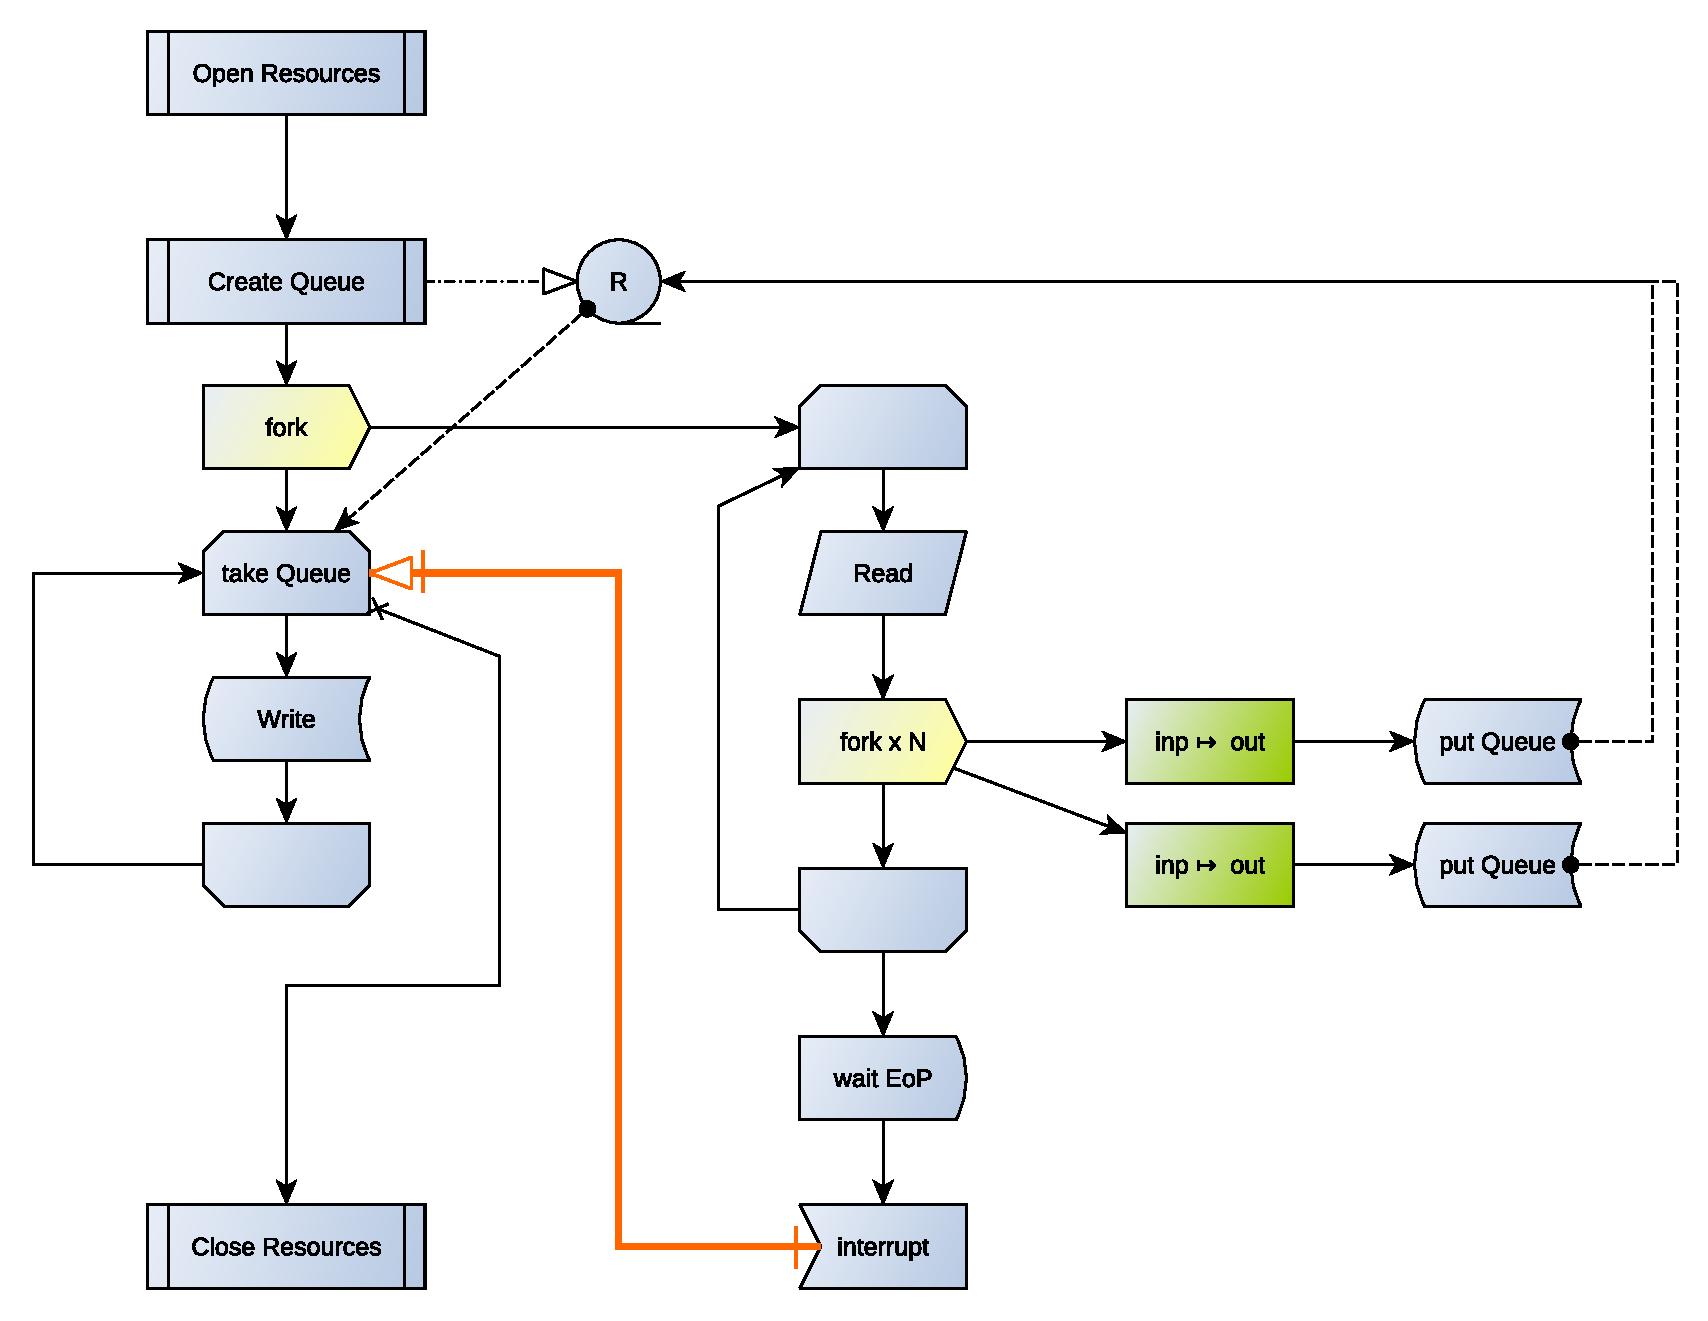
\includegraphics[scale=0.4]{../img/parallel-fefw}
        \caption{Flusso elaborativo parallelo FirstEnd-FirstWrite} \label{fig:fefw}
    \end{center}
\end{figure}
%--------1---------2---------3---------4---------5---------6---------7---------8

\subsection{First End First Write} \label{sec:fefw}
%--------1---------2---------3---------4---------5---------6---------7---------8
Questa implementazione viene usata quando l'\,elaborazione parallela viene
invocata con la forma~\ref{lst:processTupleFEFW}.
%--------1---------2---------3---------4---------5---------6---------7---------8
\begin{elisting}[!htb]
    \begin{javacode}
        Pgm.from(src).into(snk1,snk2).forEachParallel(numTask, it -> { ... });
    \end{javacode}
    \caption{elaborazione $1\mapsto N$ (FEFW)}
    \label{lst:processTupleFEFW}
\end{elisting}
%--------1---------2---------3---------4---------5---------6---------7---------8

L'\,ela\-bo\-ra\-zio\-ne avviene come indicato nella fig.~\ref{fig:fefw}.
Si aprono tutte le risorse, di input e di output.
Si crea una coda \textsl{Block\-ing\-Que\-ue}, che verrà usata per la gestione
dell'\,output del processo elaborativo.
Viene creato un processo secondario.
Inizia un loop infinito in ascolto della coda creata,
quando viene letto un dato dalla coda, in generale un tupla di $N_O$ valori,
ogni valore viene scritto sulla risorsa di output corrispondente.
Quando il loop infinito viene interrotto, vengono chiuse le risorse.

%--------1---------2---------3---------4---------5---------6---------7---------8
Torniamo al processo secondario, questo fa il loop sui dati di input.
Per ogni dato letto viene avviato un task elaborativo,
limitando il numero massimo di task attivi a $N_T$.
Quando non ci sono più dati in input, si controlla che i task elaborativi
siano terminati, che la coda dati sia vuota, e si invia un segnale per
interrompere il loop infinito in ascolto sulla coda.

%--------1---------2---------3---------4---------5---------6---------7---------8
Il task elaborativo è composto dalla funzione che trasforma l'\,input
nell'\,output, la $\lambda$-function del \textsl{forEachParallel}, e
dalla scrittura dell'\,output sulla coda dati.

%--------1---------2---------3---------4---------5---------6---------7---------8
Un punto delicato di questa gestione parallela è la parte finale del processo
secondario, quando sono finiti i dati di input.
Dopo che sono stati sottomessi tutti i dati di input, viene invocato lo
\textsl{shutdown} dello \textsl{ExecutorService} che gestisce i task
elaborativi, si attende fino a un tempo limite (default 30~s), dopodiché
viene invocato lo \textsl{shutdownNow} (che tenta di interrompere il task
elaborativi ancora in esecuzione).
Se la durata dei task elaborativi può essere superiore, è possibile impostare
il valore di timeout con:
%--------1---------2---------3---------4---------5---------6---------7---------8
\begin{elisting}[!htb]
    \begin{javacode}
        Pgm.from(src).into(snk1,snk2)
            .shutdownTimeout(long, TimeUnit)
            .forEachParallel(numTask, it -> { ... });
    \end{javacode}
    \caption{elaborazione $1\mapsto N$ (FEFW), con shutdown timeout}
    \label{lst:processTupleFEFW-tmo}
\end{elisting}

%--------1---------2---------3---------4---------5---------6---------7---------8
Questa implementazione non mantiene l'\,ordine originale, l'\,ordine sulle
risorse di output è comunque consistente.
Per fare un esempio, se l'\,ordine dei dati in input è $1,2,3$, sulla risorsa
di output $O_1$ posso trovare un ordine diverso $2,1,3$, ma tutte le risorse di
output hanno lo stesso ordinamento.

%--------1---------2---------3---------4---------5---------6---------7---------8
\begin{figure}[!htb]
    \begin{center}
%        
\includegraphics[width=0.8\textwidth]{parallel-fefw}
        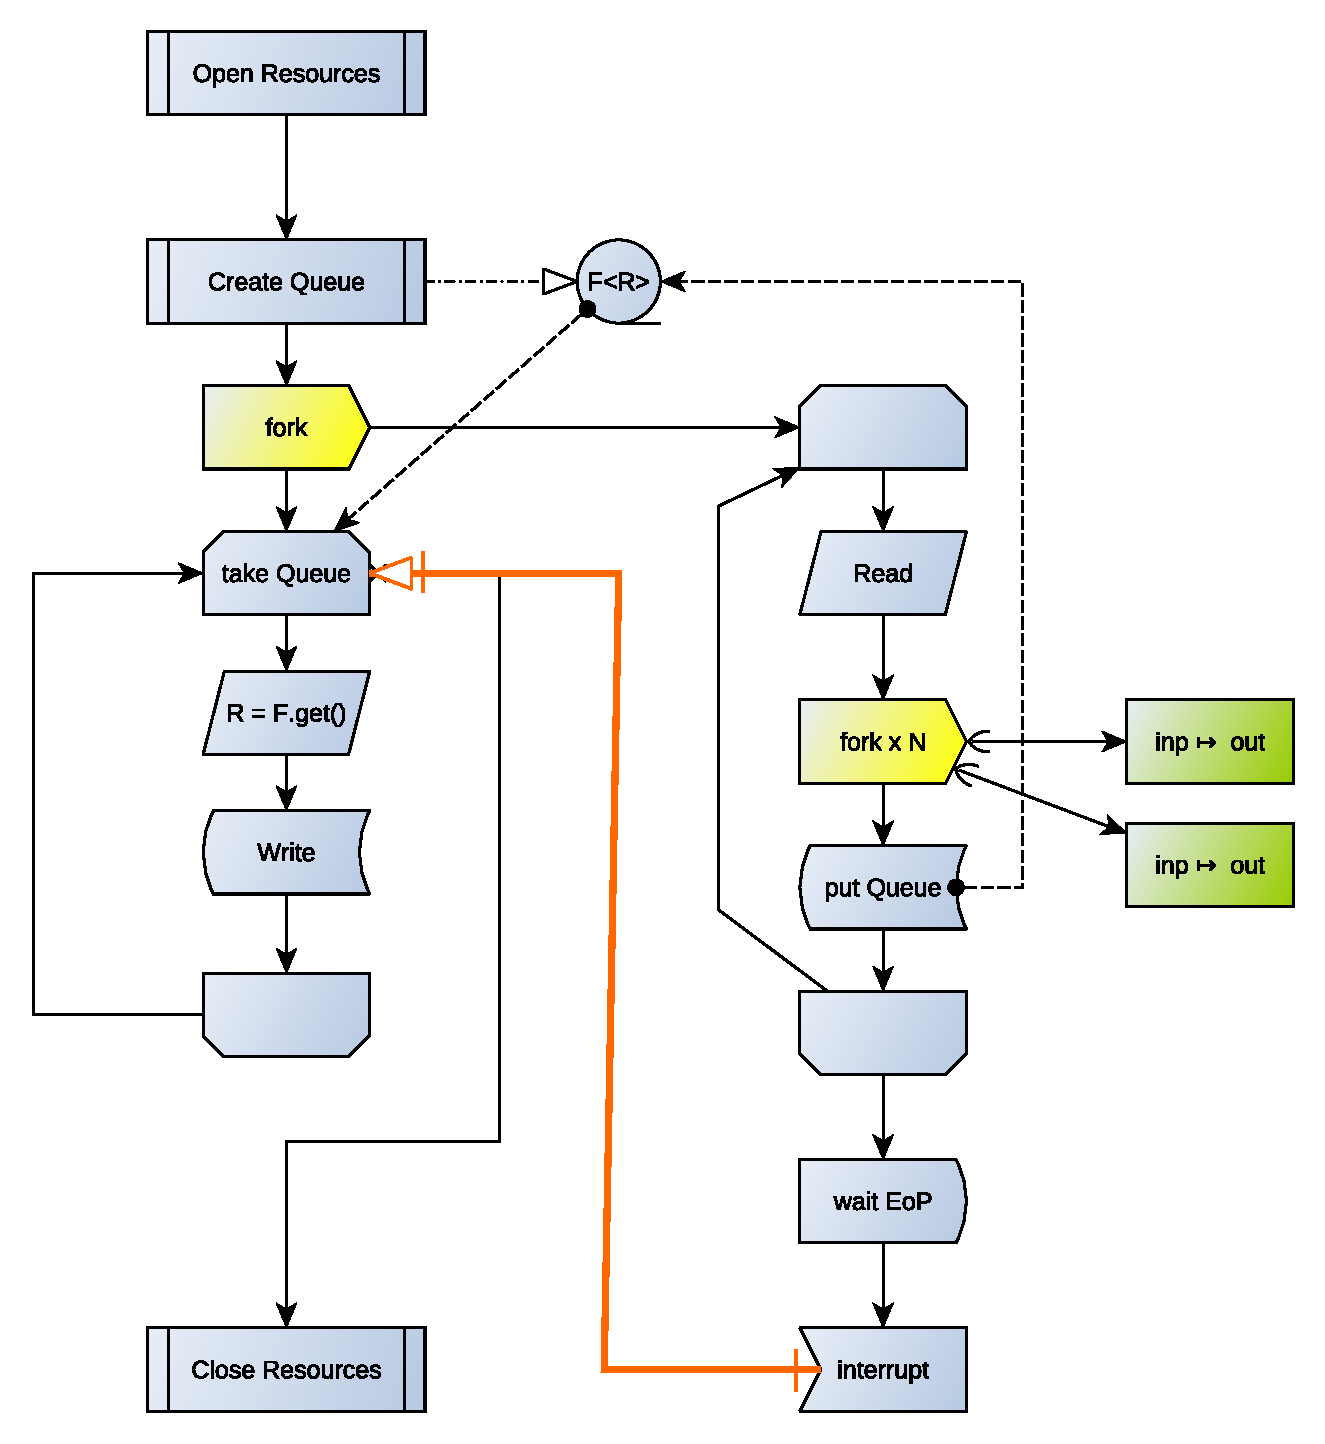
\includegraphics[scale=0.4]{../img/parallel-fsfw}
        \caption{Flusso elaborativo parallelo FirstStart-FirstWrite} \label{fig:fsfw}
    \end{center}
\end{figure}
%--------1---------2---------3---------4---------5---------6---------7---------8

\subsection{First Start First Write} \label{sec:fsfw}
%--------1---------2---------3---------4---------5---------6---------7---------8
Questa implementazione viene usata quando l'\,elaborazione parallela viene
invocata con la forma~\ref{lst:processTupleFSFW}.
%--------1---------2---------3---------4---------5---------6---------7---------8
\begin{elisting}[!htb]
    \begin{javacode}
        Pgm.from(src).into(snk1,snk2).forEachParallelFair(numTask, it -> { ... });
    \end{javacode}
    \caption{elaborazione $1\mapsto N$ (FSFW)}
    \label{lst:processTupleFSFW}
\end{elisting}
%--------1---------2---------3---------4---------5---------6---------7---------8

%--------1---------2---------3---------4---------5---------6---------7---------8
L'\,ela\-bo\-ra\-zio\-ne avviene come indicato nella fig.~\ref{fig:fsfw}.
Si aprono tutte le risorse, di input e di output.
Si crea una coda \textsl{Block\-ing\-Que\-ue}, che verrà usata per la gestione
dell'\,output del processo elaborativo.
A differenza del caso precedente, \P~\ref{sec:fefw}, la coda non ospita una tupla
con gli $N$ valori di output, ma un \textsl{Future} della tupla con gli $N$
valori di output.
Viene creato un processo secondario.
Inizia un loop infinito in ascolto della coda creata,
quando viene letto un \textsl{Future} dalla coda, vengono estratti gli $N$
valori che vengono scritti sulla risorsa di output corrispondente.
Quando il loop infinito viene interrotto, vengono chiuse le risorse.

%--------1---------2---------3---------4---------5---------6---------7---------8
Torniamo al processo secondario, questo fa il loop sui dati di input.
Per ogni dato letto viene avviato un task elaborativo,
limitando il numero massimo di task attivi a $N_T$.
La sottomissione del task elaborativo restituisce un \textsl{Future} del
risultato, e questo viene messo sulla coda dati.
Quando non ci sono più dati in input, si controlla che i task elaborativi
siano terminati, che la coda dati sia vuota, e si invia un segnale per
interrompere il loop infinito in ascolto sulla coda.

%--------1---------2---------3---------4---------5---------6---------7---------8
Il task elaborativo è semplicemente la funzione che trasforma l'\,input
nell'\,output, la $\lambda$-function del \textsl{forEachParallelFair}.

%--------1---------2---------3---------4---------5---------6---------7---------8
Se un task elaborativo è ``lento'', il loop di ascolto della coda prenderà il
\textsl{Future} del risultato, ma quando tenta di estrarre il risultato, si
ferma in attesa che il task termini.
Se il loop di ascolto si ferma, la coda si riempie, e raggiunto un valore
limite non accetta più nuovi dati.
Quando il task secondario tenta di accodare il \textsl{Future} del task appena
sottomesso, si ferma in attesa che la coda accetti nuovi dati, e non legge più
dalla risorsa di input.

%--------1---------2---------3---------4---------5---------6---------7---------8
\begin{figure}[!htb]
    \begin{center}
%        
\includegraphics[width=0.8\textwidth]{parallel-fefw}
        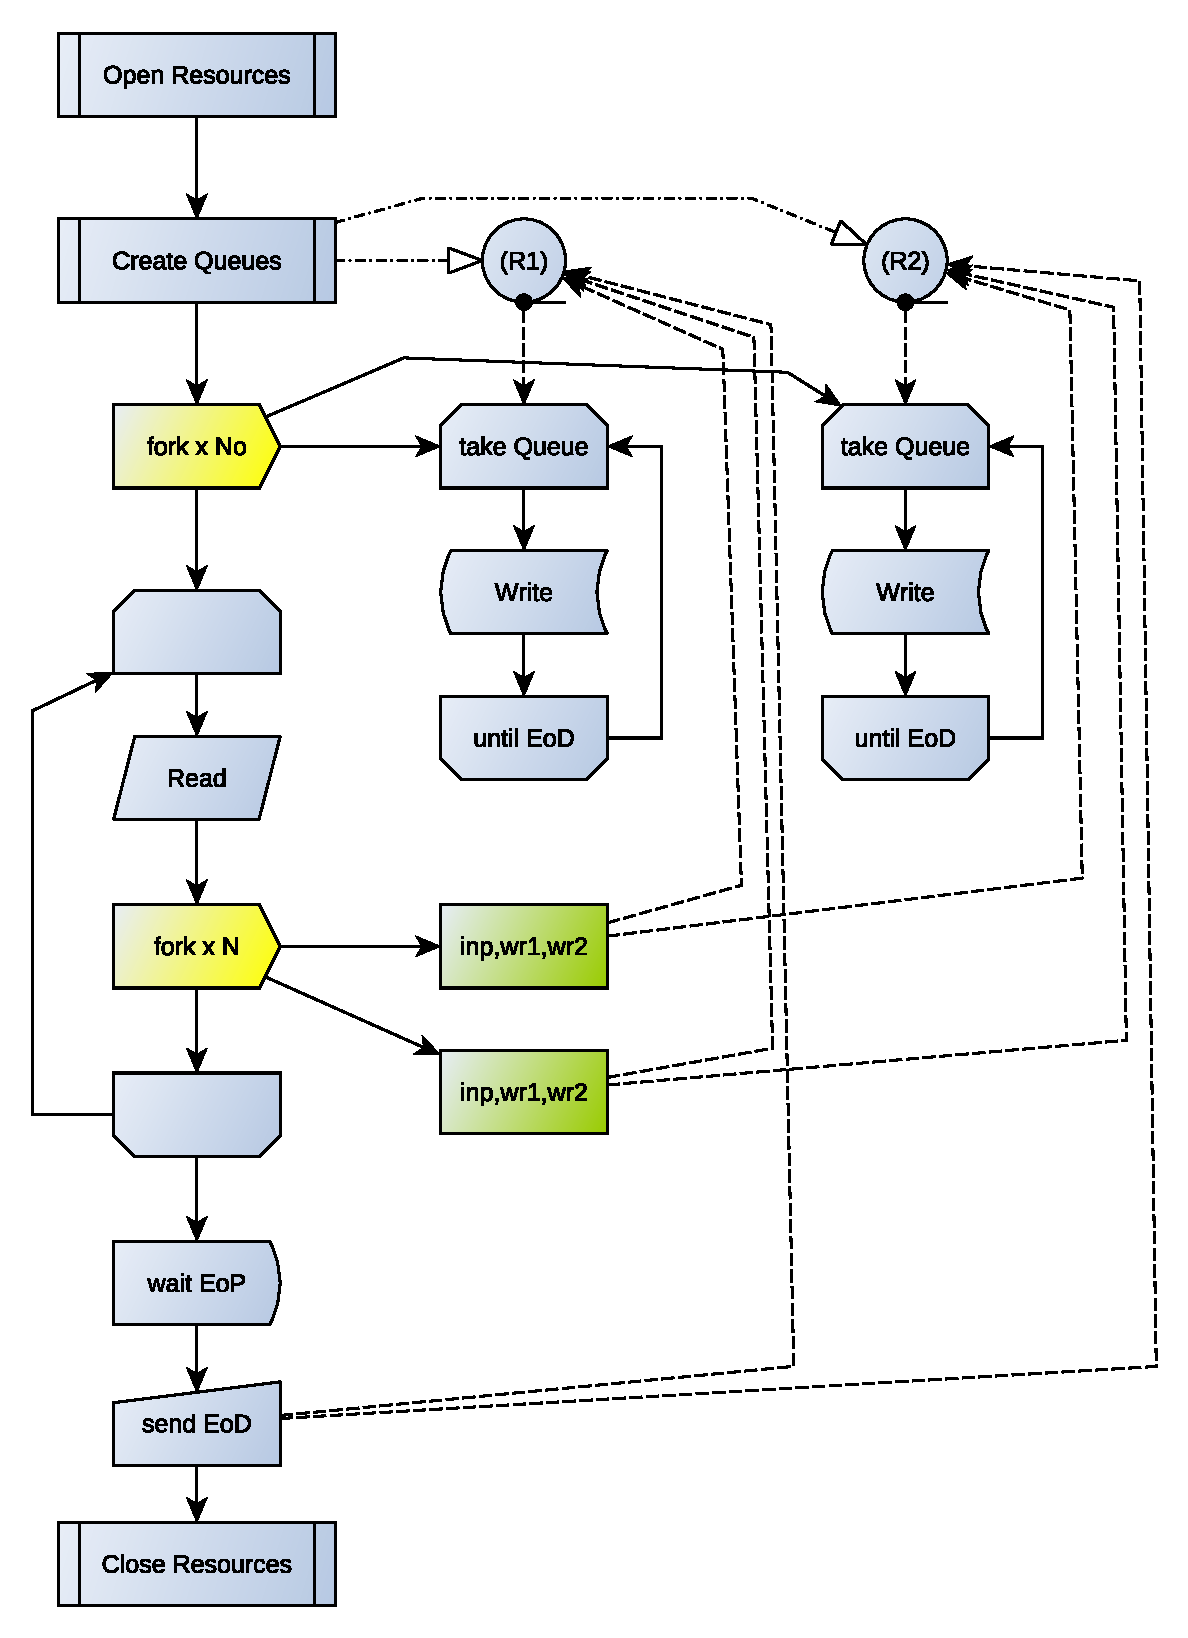
\includegraphics[scale=0.4]{../img/parallel-wr}
        \caption{Flusso elaborativo parallelo Parallel-Write} \label{fig:pwr}
    \end{center}
\end{figure}
%--------1---------2---------3---------4---------5---------6---------7---------8

\subsection{Parallel Write} \label{sec:pwr}
%--------1---------2---------3---------4---------5---------6---------7---------8
Questa implementazione viene usata quando l'\,elaborazione parallela viene
invocata con la forma~\ref{lst:processMuxWr}.
%--------1---------2---------3---------4---------5---------6---------7---------8
\begin{elisting}[!htb]
\begin{javacode}
Pgm.from(src).into(snk1,snk2).forEachParallel(numTask, (it,wr1,wr2) -> { ... });
\end{javacode}
\caption{elaborazione $1,W_1,\dots,W_N$ (PMW)}
\label{lst:processMuxWr}
\end{elisting}
%--------1---------2---------3---------4---------5---------6---------7---------8
L'\,ela\-bo\-ra\-zio\-ne avviene come indicato nella fig.~\ref{fig:pwr}.
Si aprono tutte le risorse, di input e di output.
Per ogni risorsa di output viene creata una coda \textsl{Block\-ing\-Que\-ue}
dedicata.
Per ogni risorsa di output viene creato un task in ascolto sulla coda della
rispettiva risorsa.
Queste code non ospitano il tipo dati della risorsa di output, ma una classe che
\textsl{Wrap}-pa del tipo dati, la classe \textsl{Wrap} permette di inviare un
dato speciale che indica di terminare il loop di ascolto e il task.
Inizia il loop di lettura dei dati di input.
Per ogni dato letto viene avviato un task elaborativo,
limitando il numero massimo di task attivi a $N_T$.
Quando non ci sono più dati in input, si controlla che i task elaborativi
siano terminati, che le code dati siano vuote, e per ogni coda dati viene
inviato un valore speciale che farà terminare il task di ascolto.
Si controlla che i task di ascolto siano terminati, e si chiude le risorse.

%--------1---------2---------3---------4---------5---------6---------7---------8
Il task elaborativo è semplicemente la $\lambda$-function del
\textsl{forEachParallel}.
Da osservare che la $\lambda$-function \textit{scrive} il tipo dati della classe di
output, ma sulla coda corrispondente ci finisce una versione \textsl{Wrap}-pata.

%--------1---------2---------3---------4---------5---------6---------7---------8
I task di ascolto sulle code, leggono il dato e lo scrivono sulla risorsa, se il
dato letto è il valore speciale che indica la fine-dati, escono dal loop di
ascolto e terminano il task.

%--------1---------2---------3---------4---------5---------6---------7---------8
Questa implementazione non mantiene l'\,ordine originale, inoltre l'\,ordine
sulle risorse di output potrebbe essere inconsistente.
Per fare un esempio, se l'\,ordine dei dati in input è $1,2,3$, sulla risorsa di
output $O_1$ posso trovare $2,1,3$ e sulla risorsa di output $O_2$ posso trovare
un altro ordine $1,3,2$.

%--------1---------2---------3---------4---------5---------6---------7---------8

\subsection{Async Single Write} \label{sec:asw}
%--------1---------2---------3---------4---------5---------6---------7---------8
Quando il processo elaborativo di trasformazione dell'\,input negli $N$ valori
di output è implementato mediante una funzione asincrona, lis.~\ref{lst:taskAsw}
%--------1---------2---------3---------4---------5---------6---------7---------8
\begin{elisting}[!htb]
\begin{javacode}
    @Async("TaskExecutor")
    public Future<Tuple2<O1,O2>> workerTask(I i) { ... }
\end{javacode}
\caption{task $1\mapsto N$ asincrono (ASW)}
\label{lst:taskAsw}
\end{elisting}
%--------1---------2---------3---------4---------5---------6---------7---------8
è possibile utlizzare l'\,elaborazione parallela nella
forma~\ref{lst:processAsw}.
%--------1---------2---------3---------4---------5---------6---------7---------8
\begin{elisting}[!htb]
\begin{javacode}
Pgm.from(src).into(snk1,snk2).forEachAsync(numTask, that::workerTask);
\end{javacode}
\caption{elaborazione $1\mapsto N$ asincrona (ASW)}
\label{lst:processAsw}
\end{elisting}
%--------1---------2---------3---------4---------5---------6---------7---------8
Il flusso elaborativo è simile a quello della fig.~\ref{fig:fsfw}, l'\,unica
differenza è che anziché creare un \textsl{ExecutorService} per gestire la
sottomissione dei task elaborativi, ne viene usato uno esterno (quello di
\textit{Spring}), e alla fine dei dati di input non viene invocato il suo
\textsl{shutdown}, ma semplicemente si monitora che tutti i task elaborativi
siano terminati.

%--------1---------2---------3---------4---------5---------6---------7---------8
Questa implementazione mantiene in output l'\,ordine dei dati di input.

%--------1---------2---------3---------4---------5---------6---------7---------8

\subsection{Async Parallel Write} \label{sec:apw}
%--------1---------2---------3---------4---------5---------6---------7---------8
Quando il processo elaborativo che prende il valore di input e \textit{scrive}
gli $N$ valori di output è implementato mediante una funzione asincrona,
lis.~\ref{lst:taskApw}
%--------1---------2---------3---------4---------5---------6---------7---------8
\begin{elisting}[!htb]
\begin{javacode}
    @Async("TaskExecutor")
    public Future<?> workerTask(I i, Consumer<O1> wr1, Consumer<O2> wr2) { ... }
\end{javacode}
\caption{task $1,W_1,\dots,W_N$ asincrono (APW)}
\label{lst:taskApw}
\end{elisting}
%--------1---------2---------3---------4---------5---------6---------7---------8
è possibile utlizzare l'\,elaborazione parallela nella
forma~\ref{lst:processApw}.
%--------1---------2---------3---------4---------5---------6---------7---------8
\begin{elisting}[!htb]
\begin{javacode}
Pgm.from(src).into(snk1,snk2).forEachAsync(numTask, that::workerTask);
\end{javacode}
\caption{Elaborazione $1,W_1,\dots,W_N$ asincrona (APW)}
\label{lst:processApw}
\end{elisting}
%--------1---------2---------3---------4---------5---------6---------7---------8
Il flusso elaborativo è simile a quello della fig.~\ref{fig:pwr}, l'\,unica
differenza è che anziché creare un \textsl{ExecutorService} per gestire la
sottomissione dei task elaborativi, ne viene usato uno esterno (quello di
\textit{Spring}), e alla fine dei dati di input non viene invocato il suo
\textsl{shutdown}, ma semplicemente si monitora che tutti i task elaborativi
siano terminati.

%--------1---------2---------3---------4---------5---------6---------7---------8
Questa implementazione non mantiene l'\,ordine dei dati, vedi fine
\P~\ref{sec:pwr}.

\section{Sorgente dati --- \texttt{SourceResource}} \label{sec:srcRes}
%--------1---------2---------3---------4---------5---------6---------7---------8
Una generica sorgente dati è una classe che implementa l'\,interfaccia
\texttt{SourceResource}, vedi lis.~\ref{lst:srcRef}, dove il metodo \texttt{get}
fornisce la risorsa \texttt{U} che può essere usata in un
\texttt{try-with-resources}, e i metodi \texttt{iterator} e \texttt{supplier}
permettono di \textsl{leggere} gli elementi mediante un loop\footnote{%
    uso di una \texttt{SourceResource} con un \texttt{Iterator}:
    \begin{javacode}
        try (U u = source.get()) {
        Iterator<I> iterator = source.iterator(u);
        while (iterator.hasNext()) {
            I i = iterator.next();
            // TODO
        }
    }
    \end{javacode}
} o dei supplier\footnote{%
    uso di una \texttt{SourceResource} con un \texttt{Supplier}:
    \begin{javacode}
        try (U u = source.get()) {
        Supplier<I> supplier = source.supplier(u);
        I i = supplier.get();
        while (i != null) {
            // TODO
            i = supplier.get();
        }
    }
    \end{javacode}
}.
%--------1---------2---------3---------4---------5---------6---------7---------8

%--------1---------2---------3---------4---------5---------6---------7---------8
\begin{elisting}[!htb]
\begin{javacode}
public interface SourceResource<U extends AutoCloseable, I> {
    U get();
    Iterator<I> iterator(U u);
    Supplier<I> supplier(U u);
}
\end{javacode}
\caption{Metodi per aprire la risorsa e leggere i dati}
\label{lst:srcRef}
\end{elisting}
%--------1---------2---------3---------4---------5---------6---------7---------8

%--------1---------2---------3---------4---------5---------6---------7---------8
L'\,interfaccia oltre a indicare i metodi di istanza offre dei costruttori
statici facilitare l'\,implementazione della interfaccia.
%--------1---------2---------3---------4---------5---------6---------7---------8

%--------1---------2---------3---------4---------5---------6---------7---------8
\begin{elisting}[!htb]
\begin{javacode}
public interface SourceResource<U extends AutoCloseable, I> {
    static SourceResource<BufferedReader, String> bufferedReader(File file, Charset cs, Runnable inc);
    static SourceResource<BufferedReader, String> bufferedReader(File file, Runnable inc);
    static SourceResource<BufferedReader, String> bufferedReader(File file, Charset cs);
    static SourceResource<BufferedReader, String> bufferedReader(File file);
}
\end{javacode}
\caption{Metodi creare una risorsa \texttt{SourceResource<BufferedReader, String>}}
\label{lst:srcRefBr}
\end{elisting}
%--------1---------2---------3---------4---------5---------6---------7---------8
%--------1---------2---------3---------4---------5---------6---------7---------8
Se leggiamo un file, una riga per volta, possiamo usare il metodo statico
\texttt{bufferedReader}, sono disponibili 4 varianti, lis.~\ref{lst:srcRefBr}.
L'\,argomento \texttt{file} è obbligatorio, è possibile indicare un charset per
la lettura del file, ed è possibile indicare un'\,azione da eseguire dopo aver
letto una riga dal file (normalmente un contatore per le statistiche di
esecuzione).
%--------1---------2---------3---------4---------5---------6---------7---------8

%--------1---------2---------3---------4---------5---------6---------7---------8
\begin{elisting}[!htb]
\begin{javacode}
public interface SourceResource<U extends AutoCloseable, I> {
    static <I> SourceResource<BufferedReader, I> bufferedReader(File file, Function<String,I> dec,
                                                                Charset cs, Runnable inc);
    static <I> SourceResource<BufferedReader, I> bufferedReader(File file, Function<String,I> dec, Charset cs);
    static <I> SourceResource<BufferedReader, I> bufferedReader(File file, Function<String,I> dec, Runnable inc);
    static <I> SourceResource<BufferedReader, I> bufferedReader(File file, Function<String,I> dec);
}
\end{javacode}
\caption[Metodi creare una risorsa \texttt{SourceResource<BufferedReader,I>}
con funzione di decodifica]{Metodi creare una risorsa \texttt{SourceResource<BufferedReader,I>}
con funzione di decodifica \texttt{String}~$\mapsto$~\texttt{I}}
\label{lst:srcRefBrDec}
\end{elisting}
%--------1---------2---------3---------4---------5---------6---------7---------8
Se il file viene letto una riga per volta, e la riga viene deserializzata nella
classe dati, può essere usato un costruttore nella forma
lis.~\ref{lst:srcRefBrDec}, che sono analoghi alla forma precedente, ma hanno
la funzione di decodifica in modo che l'\,iterator o il supplier forniscano
direttamente la classe dati.
%--------1---------2---------3---------4---------5---------6---------7---------8

%--------1---------2---------3---------4---------5---------6---------7---------8
\begin{elisting}[!htb]
\begin{javacode}
public interface SourceResource<U extends AutoCloseable, I> {
    static <U extends AutoCloseable, I> SourceResource<U, I> fromIterator(Supplier<U> ctor,
                                                                          Function<U, Iterator<I>> reader);
    static <U extends AutoCloseable & Iterable<I>, I> SourceResource<U, I> fromIterator(Supplier<U> ctor);
    static <I> SourceResource<?, I> fromIterator(Iterable<I> iterable);
}
\end{javacode}
\caption{Metodi per creare una origine dati da un iterator}
\label{lst:srcRefIter}
\end{elisting}
%--------1---------2---------3---------4---------5---------6---------7---------8
Infine esistono i costruttori statici generici mediante \texttt{Iterator},
lis.~\ref{lst:srcRefIter}, e \texttt{Supplier}, lis.~\ref{lst:srcRefSupp}.
%--------1---------2---------3---------4---------5---------6---------7---------8

%--------1---------2---------3---------4---------5---------6---------7---------8
\begin{elisting}[!htb]
\begin{javacode}
public interface SourceResource<U extends AutoCloseable, I> {
    static <U extends AutoCloseable, I> SourceResource<U, I> fromSupplier(
        Supplier<U> ctor, Function<U, Supplier<I>> reader);
    static <U extends AutoCloseable & Supplier<I>, I> SourceResource<U, I> fromSupplier(Supplier<U> ctor);
}
\end{javacode}
\caption{Metodi per creare una origine dati da un supplier}
\label{lst:srcRefSupp}
\end{elisting}
%--------1---------2---------3---------4---------5---------6---------7---------8


\section{Destinazione dati --- \texttt{SinkResource}} \label{sec:snkRes}
%--------1---------2---------3---------4---------5---------6---------7---------8
Una generica destinazione dati è una classe che implementa l'\,interfaccia
\texttt{SinkResource}, vedi lis.~\ref{lst:snkRef}, dove il metodo \texttt{get}
fornisce la risorsa \texttt{U} che può essere usata con un
\texttt{try-with-resources} ed il metodo \texttt{accept} scrive\footnote{%
    uso di una \texttt{SinkResource}:
    \begin{javacode}
        try (T t = sink.get()) {    // open resource
        O o = // TODO
        sink.accept(t, o);      // write data
    }
    \end{javacode}
} il dato.
%--------1---------2---------3---------4---------5---------6---------7---------8
L'\,interfaccia oltre a indicare i metodi di istanza offre dei costruttori
statici per facilitare l'\,implementazione dell'\,interfaccia.
%--------1---------2---------3---------4---------5---------6---------7---------8

%--------1---------2---------3---------4---------5---------6---------7---------8
\begin{elisting}[!htb]
\begin{javacode}
public interface SinkResource<U extends AutoCloseable, O> {
    U get();
    void accept(U u, O o);
}
\end{javacode}
\caption{Metodi per aprire la risorsa e scrivere i dati}
\label{lst:snkRef}
\end{elisting}
%--------1---------2---------3---------4---------5---------6---------7---------8

%--------1---------2---------3---------4---------5---------6---------7---------8
Se la risorsa è un file e viene scritta una riga per volta possono essere usato
il metodo statico \texttt{bufferedWriter}, sono disponibili 4 varianti,
lis.~\ref{lst:snkRefBw}. L'\,argomento \texttt{file} è obbligatorio, è possibile
indicare il charset per la scrittura del file, e una azione da eseguire dopo
aver scritto la riga del file (normalmente un contatore per le statistiche di
esecuzione).
%--------1---------2---------3---------4---------5---------6---------7---------8

%--------1---------2---------3---------4---------5---------6---------7---------8
\begin{elisting}[!htb]
\begin{javacode}
public interface SinkResource<U extends AutoCloseable, O> {
    static SinkResource<BufferedWriter, String> bufferedWriter(File file, Charset cs, Runnable inc);
    static SinkResource<BufferedWriter, String> bufferedWriter(File file, Runnable inc);
    static SinkResource<BufferedWriter, String> bufferedWriter(File file, Charset cs);
    static SinkResource<BufferedWriter, String> bufferedWriter(File file);
}
\end{javacode}
\caption{Metodi per creare una risorsa \texttt{SinkResource<BufferedWriter, String>}}
\label{lst:snkRefBw}
\end{elisting}
%--------1---------2---------3---------4---------5---------6---------7---------8

%--------1---------2---------3---------4---------5---------6---------7---------8
Se la riga sul file rappresenta la serializzazione di un oggetto, possono essere
usati i costruttori statici nella forma lis.~\ref{lst:snkRefBwEnc}, che sono
analoghi alla forma precedente, ma hanno la funzione di codifica della classe
in stringa, in modo che il \textit{writer} possa scrivere direttamente la classe
dati.
%--------1---------2---------3---------4---------5---------6---------7---------8

%--------1---------2---------3---------4---------5---------6---------7---------8
\begin{elisting}[!htb]
\begin{javacode}
public interface SinkResource<U extends AutoCloseable, O> {
    static <O> SinkResource<BufferedWriter, O> bufferedWriter(File file, Function<O,String> enc, Charset cs,
                                                              Runnable inc);
    static <O> SinkResource<BufferedWriter, O> bufferedWriter(File file, Function<O,String> enc, Charset cs);
    static <O> SinkResource<BufferedWriter, O> bufferedWriter(File file, Function<O,String> enc, Runnable inc);
    static <O> SinkResource<BufferedWriter, O> bufferedWriter(File file, Function<O,String> enc);
}
\end{javacode}
\caption[Metodi per creare una risorsa \texttt{SinkResource<BufferedWriter,O>}
con funzione di codifica]{Metodi per creare una risorsa \texttt{SinkResource<BufferedWriter,O>}
con funzione di codifica \textit{O}~$\mapsto$~\texttt{String}}
\label{lst:snkRefBwEnc}
\end{elisting}
%--------1---------2---------3---------4---------5---------6---------7---------8

%--------1---------2---------3---------4---------5---------6---------7---------8
Infine esistono i costruttori statici generici, lis.~\ref{lst:snkRefGen}.
Il parametro \texttt{action} indica una azione che viene eseguita dopo la
scrittura del dato (normalmente un contatore per le statistiche di esecuzione).
%--------1---------2---------3---------4---------5---------6---------7---------8

%--------1---------2---------3---------4---------5---------6---------7---------8
\begin{elisting}[!htb]
\begin{javacode}
public interface SinkResource<U extends AutoCloseable, O> {
    static <U extends AutoCloseable, O> SinkResource<U, O> of(Supplier<U> ctor, BiConsumer<U, O> writer);
    static <U extends AutoCloseable, O> SinkResource<U, O> of(Supplier<U> ctor, BiConsumer<U, O> writer,
                                                              Runnable action);
    static <O> SinkResource<?, O> of(Consumer<O> writer);
    static <O> SinkResource<?, O> of(Consumer<O> writer, Runnable action);
}
\end{javacode}
\caption{Metodi per creare una risorsa \texttt{SinkResource} generica}
\label{lst:snkRefGen}
\end{elisting}
%--------1---------2---------3---------4---------5---------6---------7---------8

\subsection{Destinazione dati --- \texttt{SinkBufResource}} \label{sec:snkBufRes}
%--------1---------2---------3---------4---------5---------6---------7---------8
A volte una destinazione dati non \textit{scrive} immediatamente i dati che 
riceve, ma gli accumula in un buffer, e la scrittura avviene al raggiungimento
di un limite del buffer o prima della chiusura della risorsa.
Questa implementazione in generale è più performante rispetto alla scrittura 
immediata.

%--------1---------2---------3---------4---------5---------6---------7---------8
Quando si hanno più destinazioni dati, in generale, le soglie dei rispettivi
buffer non vengono raggiunte in modo sincrono, e i dati vengono scritti, 
temporaneamente, in modo inconsistente.
Questo non è un problema se le risorse sono files, ma se le risorse sono update
(insert) batch su tabelle diverse, collegate, di un database, potrebbe essere 
un problema.

%--------1---------2---------3---------4---------5---------6---------7---------8
L'\,interfaccia \texttt{SinkBufResource} è banalmente una estensione della 
interfaccia \texttt{SinkResource}, che rispetto a questa, ha in più il metodo
\texttt{flush()} che permette di forzare la scritura del buffer.
Questo permette di impostare i legami delle risorse e scrivere i dati sulle 
risorse collegate in modo consistente.

%--------1---------2---------3---------4---------5---------6---------7---------8
\begin{elisting}[!htb]
\begin{javacode}
public interface SinkBufResource<U extends AutoCloseable, O> extends SinkResource<U, O> {
	void flush();
	static <U extends AutoCloseable, O>
    SinkBufResource<U, O> of(Supplier<U> ctor, BiConsumer<U, O> writer, Consumer<U> flusher);
    static <U extends AutoCloseable, O>
    SinkBufResource<U, O> of(Supplier<U> ctor, BiConsumer<U, O> writer, Consumer<U> flusher, Runnable action);
	...
}
\end{javacode}
\caption{Metodi per creare una risorsa \texttt{SinkBufResource} generica}
\label{lst:snkBufResGen}
\end{elisting}
%--------1---------2---------3---------4---------5---------6---------7---------8

%--------1---------2---------3---------4---------5---------6---------7---------8
\begin{elisting}[!htb]
\begin{javacode}
public interface SinkBufResource<U extends AutoCloseable, O> extends SinkResource<U, O> {
	...
    static SinkBufResource<BufferedWriter, String> bufferedWriter(File file, Charset cs, Runnable inc);
    static SinkBufResource<BufferedWriter, String> bufferedWriter(File file, Runnable inc);
    static SinkBufResource<BufferedWriter, String> bufferedWriter(File file, Charset cs);
    static SinkBufResource<BufferedWriter, String> bufferedWriter(File file);
	...
}
\end{javacode}
\caption{Metodi per creare una risorsa \texttt{SinkBufResource<BufferedWriter, String>}}
\label{lst:snkBufResStr}
\end{elisting}
%--------1---------2---------3---------4---------5---------6---------7---------8

%--------1---------2---------3---------4---------5---------6---------7---------8
\begin{elisting}[!htb]
\begin{javacode}
public interface SinkBufResource<U extends AutoCloseable, O> extends SinkResource<U, O> {
	...
    static <O> SinkBufResource<BufferedWriter, O> bufferedWriter(
    		File file, Function<O, String> enc, Charset cs, Runnable inc);
    static <O> SinkBufResource<BufferedWriter, O> bufferedWriter(
    		File file, Function<O, String> enc, Runnable inc);
    static <O> SinkBufResource<BufferedWriter, O> bufferedWriter(File file, Function<O, String> enc, Charset cs);
    static <O> SinkBufResource<BufferedWriter, O> bufferedWriter(File file, Function<O, String> enc);
}
\end{javacode}
\caption{Metodi per creare una risorsa \texttt{SinkBufResource<BufferedWriter, O>} con funzione di codifica}
\label{lst:snkBufResFcn}
\end{elisting}
%--------1---------2---------3---------4---------5---------6---------7---------8

